% 第3章第1节：场、方程与边界数据（从状态向量到空间场；初值、边界条件与解的含义）。

\section{场、方程与边界数据}
\label{sec:pde-fields-boundary-data}

本节先说明未知量怎样从有限个坐标变成空间上的函数，再区分只受空间约束的静态场与随时间变化的演化场。随后讨论边界上可以规定哪些数据、初值与边界在交接处怎样协调，以及“解”可以有几种含义。后面四节分别研究的Poisson、热、输运与波动方程，都要先在这里确定数据和解的意义。

\subsection{从状态向量到空间场}
\label{sec:pde-state-to-field}

\paragraph{一根细棒上的温度}
设一根长为$1$的细棒占据区间$[0,1]$，两端浸在冰水中。棒很细，同一横截面上的温度可以看成相同，于是在时刻$t$，位置$x$处只有一个温度$u(x,t)$。固定时刻$t$，整条曲线$x\mapsto u(x,t)$就是棒在这一时刻的状态。它不是一个数，也不是有限个数，而是区间上的一个函数，我们称这样随位置变化的量为\term{场}（field）。

图~\ref{fig:pde-rod-snapshots}画出了一个初始有两个热点的温度场在几个时刻的样子。蓝色曲线是初始温度，随着时间推移，两个尖峰变矮变宽，最后连成一个平缓的拱形，两端始终保持零度。在$t=0.004$这条曲线上，我们还在$11$个等距网格点处取了样：这$11$个温度组成的向量正是上一章意义下的有限维状态。它只是场的一个近似表示，网格点之间的温度、尖峰的确切形状都被丢掉了；第~\ref{sec:pde-discretization}节再研究这种近似何时可靠。

\begin{figure}[!htb]
  \centering
  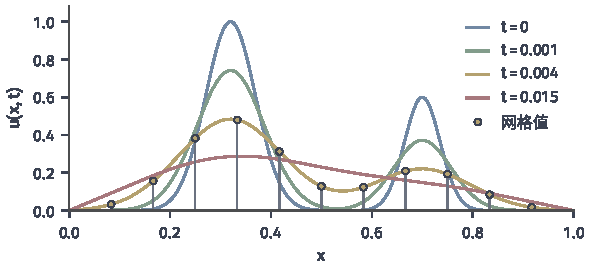
\includegraphics[width=100mm]{figures/03-optimization-evolution-and-signals/02-processes-and-trajectory-evolution/matplotlib/pde-rod-snapshots/figure.pdf}
  \caption{细棒温度场的几个时刻。方程为$u_t=u_{xx}$，两端温度保持为零，初始温度在$x=0.32$与$x=0.7$处各有一个热点。四条曲线是同一个场在不同时刻的整体形状；圆点是$t=0.004$时在$x_j=j/12$（$j=1,\ldots,11$）处取的样，组成一个$11$维向量。曲线由$300$项正弦级数计算。}
  \label{fig:pde-rod-snapshots}
\end{figure}

\paragraph{偏导数读出两种变化}
场$u(x,t)$有两个自变量，变化也有两个方向。固定时刻、沿棒移动，$\partial_xu=u_x$是温度曲线在$x$处的斜率：斜率为正说明右边更热，热量会从右向左流。固定位置、让时间前进，$\partial_tu=u_t$是这一点温度上升或下降的速率。上一章的状态方程规定$\dot{\bm x}$怎样由$\bm x$决定；对场而言，我们要规定$u_t$怎样由$u$在空间上的形状决定，而形状要用$u_x$、$u_{xx}$等空间偏导数来描述。

二阶偏导数有一个直接的读法。设$u$对$x$三次连续可微，由Taylor展开，
\begin{equation}
  \frac{u(x+h,t)+u(x-h,t)}{2}-u(x,t)=\frac{h^2}{2}u_{xx}(x,t)+o(h^2),\qquad h\to0 .
  \label{eq:pde-neighbor-average}
\end{equation}
左边是两侧邻点的平均值减去当前值。所以$u_{xx}>0$表示这一点比邻居的平均值低，曲线在这里向上弯；$u_{xx}<0$表示这一点比邻居高，处在一个凸起上。在$d$维中，Laplace算子$\Delta u=\sum_{i=1}^d\partial_{x_i}^2u$在同样的意义下比较一点的值与周围小球面上的平均值。

\paragraph{静态场与演化场}
并非所有场都随时间变化。一块薄板在固定热源下达到的稳态温度、一张绷紧的膜在固定载荷下的位移、电荷分布产生的静电势，都只依赖位置。这类\term{静态场}（stationary field）只受空间方程约束，例如稳态温度满足$-\Delta u=f$，其中$f$是热源密度；它没有初始时刻，也不需要初值。随时间变化的\term{演化场}（evolving field）则还需要一个起点：热方程要给出初始温度$u(\cdot,0)$，波动方程还要给出初始速度。初值本身是一个函数，这是“状态是函数”的直接后果。

上面这些方程有一个共同的形式：在每一点处，未知函数与它的有限个偏导数满足一个关系。

\begin{definition}[偏微分方程]
\label{def:pde-pde}
设$U\subseteq\mathbb R^n$为开集，$u:U\to\mathbb R$为未知函数。若在每一点$\bm z\in U$处，$u$与它不超过$m$阶的偏导数满足关系
\[
  F\bigl(\bm z,u(\bm z),\nabla u(\bm z),\nabla^2u(\bm z),\ldots,\nabla^mu(\bm z)\bigr)=0,
\]
且$F$确实依赖某个$m$阶偏导数，则称它是$m$阶\term{偏微分方程}（partial differential equation, PDE）。若$F$关于$u$及其各阶偏导数是仿射的，即方程可以写成$Lu=f$，其中$L$是系数只依赖$\bm z$的线性微分算子、$f$是给定函数，则称方程是线性的。
\end{definition}

对演化场，$\bm z=(\bm x,t)$同时包含空间和时间坐标，$n=d+1$。“线性”保证两个解的差满足$f=0$的方程，这一点在后面证明唯一性时反复使用。Burgers方程$u_t+uu_x=0$含有乘积$uu_x$，不是线性的；第~\ref{sec:pde-conservation}小节会看到这一差别带来的后果。

\paragraph{三种变化机制}
同一个初始形状可以按完全不同的方式演化。想象实轴上一个高为$1$的Gauss鼓包，下面三个方程各自让它怎样变化？

第一种是\term{扩散}（diffusion）：$u_t=\kappa u_{xx}$，$\kappa>0$。由式~\eqref{eq:pde-neighbor-average}，变化率正比于“邻居平均值减当前值”：鼓包顶部高于邻居，温度下降；两侧山脚低于邻居，温度上升。结果是峰变矮、形状变宽，总面积保持不变。第二种是\term{输运}（transport）：$u_t+bu_x=0$，$b$为常数。直接验证可知$u(x,t)=u_0(x-bt)$满足方程：形状不变，整体以速度$b$平移，就像河水把一团染料原样带向下游。第三种是\term{波动}（wave）：$u_{tt}=c^2u_{xx}$。这里曲率决定的是加速度而不是速度，顶部被向下拉、获得向下的速度后会越过平衡位置；在初速度为零时，鼓包分裂成两个高度减半的小鼓包，分别以速度$c$向左右跑开。

图~\ref{fig:pde-three-mechanisms}把三种机制并排画出。扩散让信息“抹平”，输运让信息“搬家”，波动让信息“分路传播”。这三幅画面贯穿本章：第~\ref{sec:pde-heat}节证明扩散抹去高频起伏、耗散能量；第~\ref{sec:pde-transport}节沿着平移的轨迹求解输运方程；第~\ref{sec:pde-wave}节说明波动以有限速度传播并保持能量。

\begin{figure*}[!htb]
  \centering
  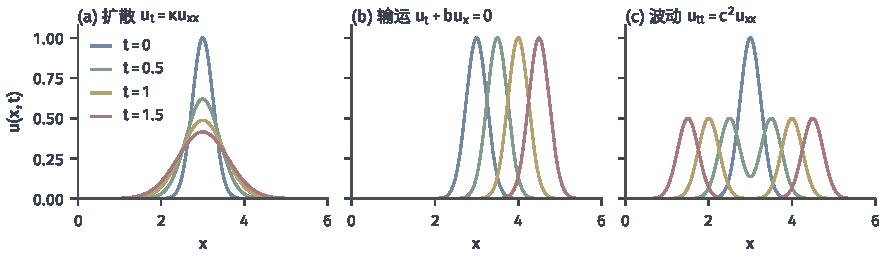
\includegraphics[width=150mm]{figures/03-optimization-evolution-and-signals/02-processes-and-trajectory-evolution/matplotlib/pde-three-mechanisms/figure.pdf}
  \caption{同一初始鼓包$u_0(x)=\exp(-(x-3)^2/(2\cdot0.25^2))$在三种方程下的演化，四种颜色依次为$t=0,0.5,1,1.5$。(a)~扩散，$\kappa=0.1$：解仍是Gauss形，方差由$0.25^2$增大为$0.25^2+2\kappa t$，峰值相应降低。(b)~输运，$b=1$：$u_0(x-t)$原样右移。(c)~波动，$c=1$，初速度为零：$\tfrac12[u_0(x-t)+u_0(x+t)]$，鼓包分为两半向两侧传播。}
  \label{fig:pde-three-mechanisms}
\end{figure*}

\paragraph{二阶方程的分类及其适用范围}
对两个自变量、常系数的二阶线性方程
\[
  a\,u_{yy}+2b\,u_{yz}+c\,u_{zz}+(\text{低阶项})=f,\qquad (a,b,c)\neq(0,0,0),
\]
常按判别式$b^2-ac$的符号分类：小于零称为\term{椭圆型}（elliptic），等于零称为\term{抛物型}（parabolic），大于零称为\term{双曲型}（hyperbolic）。名称来自二次曲线$a\xi^2+2b\xi\eta+c\eta^2=1$的形状。二维Poisson方程$-u_{yy}-u_{zz}=f$中$a=c=-1$、$b=0$，判别式为$-1$，是椭圆型；热方程$u_t-\kappa u_{xx}=0$中只有$u_{xx}$一个二阶项，判别式为$0$，是抛物型；波动方程$u_{tt}-c^2u_{xx}=0$的判别式为$c^2>0$，是双曲型。

这一分类的用处在于，同一类方程往往需要同一类数据、具有同一类性质：椭圆型方程描述平衡，在区域的整个边界上给数据；抛物型方程描述耗散的演化，给初值和边界；双曲型方程描述传播，信号沿特定方向以有限速度传递。但它只是对这种方程类的粗分，不能穷举所有偏微分方程。一阶的输运方程不在其中；系数随位置变化时，同一方程可能在一部分区域是椭圆型、在另一部分是双曲型；非线性方程的性质还可能依赖解本身。本章以四个线性代表方程为主线，分类只在相应方程处用来解释现象，不作为一般理论的出发点。

\subsection{初值、边界条件与解的含义}
\label{sec:pde-boundary-solution-meaning}

方程只规定区域内部每一点的局部关系。仅凭它，稳态热方程$-u''=0$在$(0,1)$上就有全部一次函数作为解。要让场被确定，还需要说明边界上发生了什么、演化从什么状态开始，以及在什么意义下检查“满足方程”。

\paragraph{边界上规定什么}
设$\Omega\subset\mathbb R^d$是有界开集，边界$\partial\Omega$足够规则，在几乎每个边界点有单位外法向$\bm n$。函数在边界上的\term{法向导数}（normal derivative）为$\partial_{\bm n}u=\nabla u\cdot\bm n$，它度量场沿离开区域的方向怎样变化。按热传导的语言，常见的边界条件有三类，图~\ref{fig:pde-domain-boundary}给出了示意。
\begin{itemize}
  \item \term{Dirichlet边界条件}（Dirichlet boundary condition）：$u=g$，直接规定边界上的场值，例如棒端浸在恒温水中。
  \item \term{Neumann边界条件}（Neumann boundary condition）：$\partial_{\bm n}u=g$，规定穿过边界的法向通量；$g=0$表示边界绝热。
  \item \term{Robin边界条件}（Robin boundary condition）：$\kappa\partial_{\bm n}u+\alpha u=g$，规定场值与通量之间的关系。Newton冷却定律说，向外的热流密度$-\kappa\partial_{\bm n}u$与边界温度和环境温度之差$u-u_{\mathrm{env}}$成正比，比例系数$\alpha\geq0$，整理后正是$g=\alpha u_{\mathrm{env}}$的Robin条件。
\end{itemize}
同一个区域的不同边界段可以使用不同类型，图~\ref{fig:pde-domain-boundary}左侧就把边界分成规定场值的$\Gamma_D$与规定通量的$\Gamma_N$。

\begin{figure*}[!htb]
  \centering
  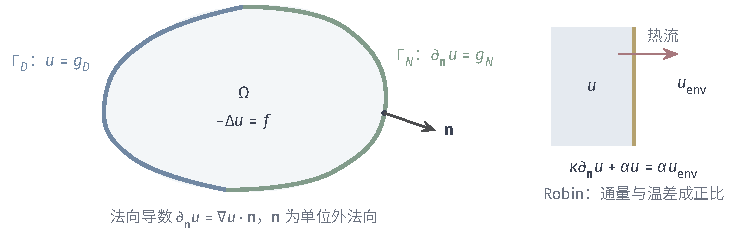
\includegraphics[width=124.5mm]{figures/03-optimization-evolution-and-signals/02-processes-and-trajectory-evolution/tikz/pde-domain-boundary/figure.pdf}
  \caption{区域与三类边界数据。左：区域$\Omega$内满足$-\Delta u=f$，边界的蓝色部分$\Gamma_D$规定场值，绿色部分$\Gamma_N$规定法向导数，箭头为一点处的单位外法向$\bm n$。右：Robin条件的物理来源，边界向外的热流与边界温度和环境温度之差成正比，系数$\alpha\geq0$。}
  \label{fig:pde-domain-boundary}
\end{figure*}

边界条件不是附加的细节，它改变解本身。下面的例子用同一个方程和同一个右端点条件，只改变左端点的类型。

\begin{example}[左端点的三种边界条件]
\label{ex:pde-three-boundary-conditions}
在$(0,1)$上考虑稳态热方程$-u''=1$，即棒内有均匀热源；右端$u(1)=0$。方程的通解是$u(x)=-x^2/2+Ax+B$。左端点的外法向指向$-x$方向，所以$\partial_{\bm n}u(0)=-u'(0)$。
\begin{itemize}
  \item Dirichlet条件$u(0)=0$：由$B=0$与$-\tfrac12+A=0$得$u(x)=x(1-x)/2$，最高温$1/8$在中点。
  \item Neumann条件$u'(0)=0$（左端绝热）：$A=0$，$B=\tfrac12$，$u(x)=(1-x^2)/2$，最高温$1/2$在绝热端。
  \item Robin条件$-u'(0)+\alpha u(0)=0$（取$\kappa=1$、$u_{\mathrm{env}}=0$）：$A=\alpha B$，再由$u(1)=0$得$B=1/(2(1+\alpha))$。取$\alpha=2$，$u(x)=-x^2/2+x/3+1/6$，左端温度$1/6$。
\end{itemize}
$\alpha=0$时Robin条件退化为Neumann条件；令$\alpha\to\infty$，$B\to0$、$A\to\tfrac12$，解趋于Dirichlet情形。
\end{example}

图~\ref{fig:pde-boundary-conditions}画出了这三条曲线。虚线是左端点的切线：Dirichlet曲线被钉在零点，Neumann曲线在左端水平，Robin曲线的左端斜率是左端值的两倍。热源相同，左端越“漏热”，整根棒越凉。

\begin{figure}[!htb]
  \centering
  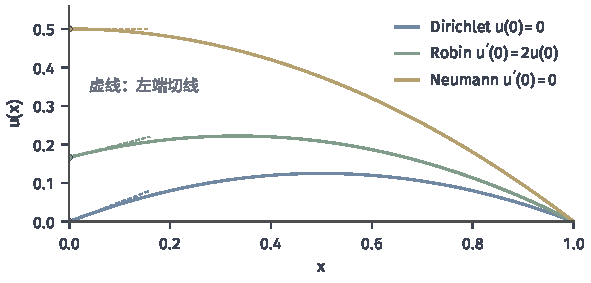
\includegraphics[width=100mm]{figures/03-optimization-evolution-and-signals/02-processes-and-trajectory-evolution/matplotlib/pde-boundary-conditions/figure.pdf}
  \caption{同一方程$-u''=1$、同一右端条件$u(1)=0$下，左端点取三种边界条件得到的解（例~\ref{ex:pde-three-boundary-conditions}）。圆点是左端值，虚线是左端切线：Dirichlet固定值为零，Neumann固定斜率为零，Robin条件$u'(0)=2u(0)$让斜率与值成比例。}
  \label{fig:pde-boundary-conditions}
\end{figure}

\paragraph{初值与边界在交接处的相容}
演化问题同时有初值和边界值，二者在区域边界与初始时刻的交接处相遇。回到细棒：若两端保持零度，而初始温度在整根棒上都是$1$，那么在角点$(x,t)=(0,0)$附近，沿$t=0$趋近得到$1$，沿$x=0$趋近得到$0$，解不可能在角点连续。第~\ref{sec:pde-heat-modes}小节会看到，这个问题对$t>0$仍有光滑的解，只是初值只能在平均意义下取到。

要让解在角点连续，至少需要\term{相容条件}（compatibility condition）$u_0(0)=g(0)$，即初值在边界上的取值与边界数据在初始时刻一致。更高的光滑性要求更多条件。例如对两端为零的热方程，边界上恒有$u=0$，于是边界上$u_t=0$；若希望$u_t$也连续到角点，方程$u_t=u_{xx}$还要求$u_0''(0)=u_0''(1)=0$。相容条件不满足时问题仍可能有解，但不连续性会从角点出发留在解中，对输运和波动方程尤其如此，它会沿着传播方向被带进区域内部。

\paragraph{经典解及其局限}
最直接的解释是逐点满足方程。对Poisson方程$-\Delta u=f$配零Dirichlet数据，\term{经典解}（classical solution）指$u\in C^2(\Omega)\cap C(\overline\Omega)$，在$\Omega$内每一点$-\Delta u=f$，在$\partial\Omega$上每一点$u=0$。这个要求在许多正常的问题上过强。

在$(0,1)$上取热源$f=2\cdot\mathbf 1_{[1/4,3/4]}$，只在中间一段加热。若$u$是经典解，则$u''=-f$在$x=1/4$两侧分别为$0$与$-2$，二阶导数不可能连续，所以经典解不存在。可是物理上应当有稳态温度：第~\ref{sec:pde-weak-form}小节将算出一个连续可微的$u$，它在除$x=1/4,3/4$外处处满足方程，跳跃只出现在二阶导数中。源集中在一点时情况更极端，一点处的点热源让温度曲线出现尖点，连一阶导数都在该点不存在。我们需要一种不要求逐点二阶导数的解释。

\paragraph{所用的Sobolev空间工具}
弱导数正是为此准备的工具。下面集中回顾本章要用的结论，它们都在固定开集$\Omega\subset\mathbb R^d$与Lebesgue测度下成立，$\langle u,v\rangle=\int_\Omega uv\,\mathrm d\bm x$与$\|u\|$分别表示$L^2(\Omega)$的内积与范数。
\begin{itemize}
  \item 若存在$v\in L^1_{\mathrm{loc}}(\Omega)$，使$\int_\Omega u\,\partial_i\varphi\,\mathrm d\bm x=-\int_\Omega v\varphi\,\mathrm d\bm x$对所有\term{测试函数}（test function）$\varphi\in C_c^\infty(\Omega)$成立，称$v$为$u$的弱导数$\partial_iu$；它在几乎处处意义下唯一。测试函数是在$\Omega$内某个紧集外为零的光滑函数，两个局部可积函数若与所有测试函数的积分都相同，则几乎处处相等。
  \item $H^1(\Omega)$由$u\in L^2(\Omega)$且各弱导数$\partial_iu\in L^2(\Omega)$的函数组成，内积$\langle u,v\rangle_{H^1}=\langle u,v\rangle+\int_\Omega\nabla u\cdot\nabla v\,\mathrm d\bm x$使它成为Hilbert空间。一维时，$H^1(a,b)$的每个元素有绝对连续的代表，满足$u(x)-u(y)=\int_y^xu'(s)\,\mathrm ds$，从而$|u(x)-u(y)|\leq|x-y|^{1/2}\|u'\|$。
  \item 设$\Omega$为有界Lipschitz区域。存在唯一的有界线性迹算子$\operatorname{Tr}:H^1(\Omega)\to L^2(\partial\Omega)$，在光滑到边界的函数上等于边界限制。$H_0^1(\Omega)$定义为$C_c^\infty(\Omega)$在$H^1$范数下的闭包，它恰好是迹为零的函数全体。若$g=\operatorname{Tr}G$，$G\in H^1(\Omega)$，则迹等于$g$的函数组成仿射集合$G+H_0^1(\Omega)$。
  \item Poincaré不等式：$\Omega$有界时，存在$C_P$使$\|u\|\leq C_P\|\nabla u\|$对所有$u\in H_0^1(\Omega)$成立；$\Omega$为有界连通Lipschitz区域时，存在$C$使$\|u-u_\Omega\|\leq C\|\nabla u\|$对所有$u\in H^1(\Omega)$成立，$u_\Omega$为均值。在区间$(0,L)$上两种情形的最优常数都是$L/\pi$。
  \item 紧嵌入：$\Omega$为有界Lipschitz区域时，$H^1(\Omega)$中的有界序列有在$L^2(\Omega)$中收敛的子列。
\end{itemize}
这些定义与定理的证明可参考\BookChapterRef{chap:weak-derivatives-sobolev}{卷二“弱导数与Sobolev空间”章}。本章用它们回答三件事：弱导数让“满足方程”可以通过与测试函数的积分来检验；迹让边界条件对$H^1$函数有意义；Poincaré不等式让梯度单独控制函数，这是后面能量估计的关键一步。

\paragraph{问题由数据、解空间与方程解释共同确定}
到这里可以说清一个偏微分方程问题由什么组成：区域与方程；源项、边界数据和初值，以及它们所属的函数空间；解所属的函数空间；“满足方程”的解释方式。后面将遇到三种解释：经典解逐点满足方程；\term{弱解}（weak solution）只要求与测试函数的积分关系成立，第~\ref{sec:pde-poisson}节为Poisson方程建立它；\term{温和解}（mild solution）用解算子与源项的积分公式定义演化，第~\ref{sec:pde-heat-semigroup}小节为热方程建立它。光滑性足够时三者一致，数据粗糙时只有较弱的解释可用。

选定这些空间以后，Hadamard提出的要求是：解存在，解唯一，并且解连续地依赖于数据，即数据的小扰动在所选范数下只引起解的小变化。三条都成立的问题称为\term{适定的}（well-posed）。三条要求都相对于所选空间而言：同一个热方程正向求解是适定的，反向求解（由今天的温度推算昨天的温度）在常用范数下却不满足连续依赖，第~\ref{sec:pde-heat-long-time}小节会给出具体的放大倍数。只写一条微分表达式，不交代数据、解空间和解释方式，问题还没有被确定。
